
% The \phantomsection command is needed to create a link to a place in the document that is not a
% figure, equation, table, section, subsection, chapter, etc.
% https://tex.stackexchange.com/questions/44088/when-do-i-need-to-invoke-phantomsection
\phantomsection

\chapter{Integer Programming}\label{chap:integer-programming}


Integer Programming (IP), a subset of mathematical programming, addresses optimization problems where decision variables are required to take on integer values.
Specifically, mixed-integer linear programming (MILP) extends this concept by encompassing the assumption that for each possible discrete decision, a (continuous) linear program has to be solved.
The complexity of MILP problems often necessitates sophisticated solution methods to find optimal or near-optimal solutions.
This chapter provides an overview of MILP problem-solving techniques, ranging from exact methods like the branch-and-bound algorithm to approaches to provide approximate solutions, such as heuristics and matheuristics.
Through these methodologies, the groundwork is laid for the subsequent discussion on deep learning-based primal heuristics, which aim to enhance the efficiency of MILP problem solving.

\section{Integer and Combinatorial Optimization}

A solution for an integer and combinatorial optimization problem is the maximum or minimum value of a multivariate function that respects a series of inequality and equality constraints and integrality restrictions on some or all variables~\cite{nemhauserIntegerCombinatorialOptimization1999}.
It is not difficult to see that integer and combinatorial optimization encompasses a wide range of problems of practical utility.
Examples include train scheduling, airline crew scheduling, production planning, electricity generation planning, and cutting problems~\cite{wolseyIntegerProgramming1998}.

Mathematical programming is a language naturally suitable to formulate integer and combinatorial optimization problems, for example, in the form
\begin{equation}\label{eq:general-ip}
    \begin{split}
	\min_{\bm{x}} \quad & f\left( \bm{x} \right) \\
	\textrm{s.t.} \quad & \bm{g}\left( \bm{x} \right) \le \bm{0} \\
	  & \bm{x} \in \Z^{n}\times \R^{p}
    ,\end{split}
\end{equation}
with $n$ integer variables and $p$ continuous variables.
Furthermore, $\bm{g}: \Z^{n}\times \R^{p} \longrightarrow \R^{m}$,  and $\bm{0}$ is a null vector of dimension $m$.
Note that maximizing a function is equivalent to minimizing its negative, and an equality constraint can be represented by two inequalities, which renders \eqref{eq:general-ip} a complete formulation.

For an integer program formulated as in \eqref{eq:general-ip}, the set \[
\mathcal{X}=\left\{ \bm{x}\in \Z^{n}\times \R^{p}: \bm{g}\left( \bm{x} \right) \le \bm{0}\right\} 
\] is named the \emph{feasible region} of the problem, and a vector $\bm{x}\in \mathcal{X}$ is a \emph{feasible solution}.
A feasible solution $\bm{x}^{*}\in \mathcal{X}$ is \emph{optimal} if, and only if, there is no other feasible solution results in a lower value of the \emph{objective function} $f: \Z^{n}\times \R^{p} \longrightarrow \R$, i.e., $\bm{x}^{*}$ is optimal $\iff f(\bm{x}^{*}) \le f(\bm{x}) ,\,\forall \bm{x}\in \mathcal{X}$.

Note that even if a problem is feasible ($\mathcal{X}\neq \varnothing$), it may not have an optimal solution, e.g., if the feasible region is unbounded and the objective function has no global minimum.
Furthermore, if an optimal solution exists, it may no be unique.
% TODO: show how a problem may have no optimal solution even if with bounded feasible region. see Nemhauser, I.4.6

Beyond the practical applications of integer programming, its computational complexity renders it an important theoretical model.
It is easy to see that integer programming is an NP-complete problem~\cite{nemhauserIntegerCombinatorialOptimization1999}.
In fact, one of Karp's 21 NP-complete problems~\cite{karpReducibilityCombinatorialProblems1972} is a special case of integer programming with no objective function (constraint satisfaction problem) and solely binary variables.

\section{Mixed-Integer Linear Programs}

MILP is a subset of IP in which the objective and the constraints are all linear functions and the problem requires integer and continuous variables.
Formally, an MILP can be formulated as 
\begin{equation}\label{eq:general-milp}
\begin{split}
    \min_{\bm{x}} \quad & \bm{c}^{T}\bm{x} \\
    \textrm{s.t.} \quad & A\bm{x} \le \bm{b} \\
	  & \bm{x} \in \Z^{n}\times \R^{p}
,\end{split}
\end{equation}
where $A\in \R^{m\times (n+p)}$ is the constraint matrix, $\bm{b}\in \R^{m}$ is the right-hand side vector, and $\bm{c}\in \R^{n+p}$ is the cost vector.
An \emph{instance} of an MILP problem is specified by a tuple  $\left( \bm{c},\bm{b},A,n \right)$.

The significance of this class of problems has already been recognized by \citeonline{dantzigSignificanceSolvingLinear1960}.
Many well-known problems can be formulated through MILP, such as the Traveling Salesperson Problem (TSP) and the map coloring problem.
Furthermore, continuous nonlinear functions can be approximated to arbitrary quality by piecewise linear functions, which admit an MILP formulation~\cite{camponogaraModelsAlgorithmsOptimal2015}.
In other words, MILP is a powerful tool for approximating optimization problems with continuous nonlinearities.

\section{Solving MILP Problems}

% TODO: solving MILP is hard, in fact, it is NP-complete, as seen Karp's 
Although MILP offers powerful models for a wide range of problems, solving such problems is unarguably hard.
In fact, the NP-complete problem formulated by \citeonline{karpReducibilityCombinatorialProblems1972} only contains linear terms, which renders it an special case of MILP and, thus, assuming P$\neq$NP, classifies MILP problems as NP-complete.
However, despite the intractable nature, there are efficient and reliable algorithms and software solutions for the computation of optimal and approximate solutions to MILP problems~\cite{bengioMachineLearningCombinatorial2021}.
Furthermore, the applications of MILP often require high-quality solutions in a limited time, which motivate the development of heuristic approaches, i.e., approaches that trade optimality (or feasibility) guarantees for a tractable running time.

\subsection{The Branch-and-Bound Algorithm}

The main idea behind the branch-and-bound algorithm is to ignore the integrality constraints of the MILP problem, solve the resulting LP, and hope that the solution has the necessary integer components~\cite{vanderbeiLinearProgrammingFoundations1998}.
If the LP relaxation\footnote{The linear programming problem obtained by ignoring the integrality constraints of an MILP is called its \emph{LP relaxation}.} of an MILP problem has an optimal solution that respects the integrality constraints, than that solution is also optimal for the original problem.
% integer solutions are naturally occuring to the LP problem on the convex hull of integer solutions for an MILP
% this is easy to see, as optimal solutions (if they exist) to LPs are always at the vertices of its feasible region (which is a polytope) and the vertices of the convex hull of an MILP all respect the original integrality constraints
However, that is not always the case.
As an example, take the MILP problem
\begin{equation}\label{eq:example-milp}
\begin{split}
    \min_{\bm{x}=(x_1,x_2)} \quad & -x_2 \\
    \textrm{s.t.} \quad & x_1 - x_2\le 0 \\
      & x_1+x_2 \le 5 \\
      & x_2 \ge 1 \\
      & \bm{x} \in \Z^2
,\end{split}
\end{equation}
for which, following the notation of \eqref{eq:general-milp}, we have \[
A=\begin{bmatrix} 1 & -1 \\ 1 & 1 \\0 & -1 \end{bmatrix}, \bm{b} = (0, 5, 0), \bm{c} = (0, -1) 
.\]
As Fig.~\ref{fig:milp-example} illustrates, the optimal solutions to this problem are $\bm{x}^{*} \in \left\{ (2,2),(3,2) \right\} $, whereas the optimal solution of its LP relaxation is $(2.5, 2.5)$. 

\begin{figure}[h]
    \centering
    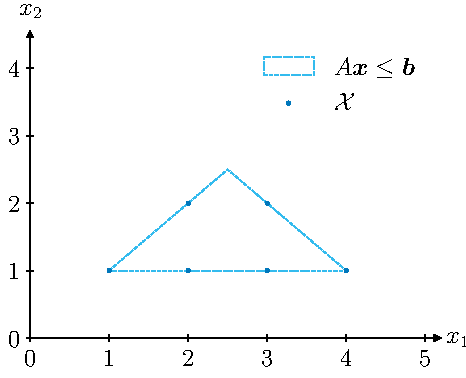
\includegraphics{pictures/milp_example_feasible_region.pdf}
    \caption{Feasible region of example MILP problem \eqref{eq:example-milp}. Dashed lines represent the feasible region of the LP relaxation.}
    \label{fig:milp-example}
\end{figure}

A naïve approach is to round the solution of the LP relaxation to the nearest integer value on the variables that violate the integrality constraints.
This strategy, however, might not even result in feasible solutions to the LP relaxation.
Note that an optimal solution to an LP is at a vertex of its feasible region, and, thus, a naïve deviation can result in an infeasible solution.


\subsection{Heuristics}

\subsection{Matheuristics}

